We now sketch the representations underpinning our approach. We define several models: an object model (partial and acquired from sensing); a model of the contact between a finger link and the object; a model of the whole hand configuration; and a model of the reach to grasp trajectory. First we describe the kernel density representation for all these models. Then we describe the surface features we use to encode some of these models. We assume that the robot's hand comprises $N_L$ rigid \emph{links}: a palm, and several phalanges or links. We denote the set of links $L =\{L_i\}$.

\subsection{Kernel Density Estimation}
\label{sec:kde}
$SO(3)$ denotes the group of rotations in three dimensions. A feature belongs to the space $SE(3) \times \mathbb R^2$, where $SE(3) = \mathbb R^3 \times SO(3)$ is the group of 3D \emph{poses}, and surface descriptors are composed of two real numbers. We extensively use probability density functions (PDFs) defined on $SE(3) \times \mathbb R^2$.  We represent these PDFs non-parametrically with a set of $K$ features (or particles) $x_j$
\begin{equation}
S = \left\lbrace x_j : x_j \in \mathbb R^3 \times SO(3) \times \mathbb R^2 \right\rbrace_{j \in [1,K]}.
\end{equation}
The probability density in a region is determined by the local density of the particles in that region. The underlying PDF is created through \emph{kernel density estimation} \cite{silverman1986a}, by assigning a kernel function $\mathcal{K}$ to each particle supporting the density, as
\begin{equation}\label{eq:d}
\pdf(x) \simeq \sum_{j=1}^K w_j \mathcal{K}(x| x_{j}, \sigma),
\end{equation}
where  $\sigma \in \mathbb R^3$ is the kernel bandwidth and $w_j \in \mathbb R^{+}$ is a weight associated to $x_j$ such that $\sum_j w_j = 1$. We use a kernel that factorises into three functions defined by the separation of $x$ into $p \in \mathbb R^3$ for position, a quaternion $q \in SO(3)$ for orientation, and $r \in \mathbb R^2$ for the surface descriptor. Furthermore, let us denote by $\mu$ another feature, and its separation into position, orientation and a surface descriptor. Finally, we denote by $\sigma$ a triplet of real numbers:
\begin{subequations}
\begin{align}
x &= (p, q, r),\\
\mu &= (\mu_p, \mu_q, \mu_r),\\
\sigma &= (\sigma_p, \sigma_q, \sigma_r).
\end{align}
\label{eq:feature}
\end{subequations}
We define our kernel as
\begin{equation}\label{eq:kernel_in_se3}
\mathcal{K}(x| \mu, \sigma) = \mathcal{N}_3(p| \mu_p, \sigma_p) \Theta(q| \mu_q, \sigma_q) \mathcal{N}_2(r| \mu_r, \sigma_r)
\end{equation}
where $\mu$ is the kernel mean point, $\sigma$ is the kernel bandwidth, $\mathcal{N}_n$ is an $n$-variate isotropic Gaussian kernel, and ${\Theta}$ corresponds to a pair of antipodal von Mises-Fisher distributions which form a Gaussian-like distribution on $SO(3)$ \cite{fisher1953a,sudderth2006a}. The value of ${\Theta}$ is given by
\begin{equation}
\Theta(q|\mu_q, \sigma_q) = C_4(\sigma_q) \frac {e^{\sigma_q \; \mu_q^T q} + e^{-\sigma_q \; \mu_q^T q}}2
\end{equation}
where $C_4(\sigma_q)$ is a normalising constant, and $\mu_q^T q$ denotes the quaternion dot product.

Using this representation, conditional and marginal probabilities can easily be computed from \eq\eqref{eq:d}. The marginal density $\pdf(r)$ is computed as
\begin{align}\label{eq:marginal}
\pdf(r) & \\
      = & \iint \sum_{j=1}^K w_j \mathcal{N}_3(p| p_i, \sigma_p) \Theta(q| q_i, \sigma_q) \mathcal{N}_2(r| r_i, \sigma_r) \textnormal{d}p\textnormal{d}q \\
      = &  \sum_{j=1}^K w_j \mathcal{N}_2(r| r_j, \sigma_r),
\end{align}
where $x_j = (p_j, q_j, r_j)$.
The  conditional density $\pdf(p,q|r)$ is given by
\begin{align}\label{eq:conditional}
\pdf(p,q|{r}) & = \frac{\pdf(p, q, {r})}{\pdf({r})} \\
                   & = \frac{\sum_{j=1}^K w_j \mathcal{N}_2({r}| r_j, \sigma_r) \mathcal{N}_3(p| p_j, \sigma_p) \Theta(q|q_j, \sigma_q)}{\sum_{j=1}^K w_j \mathcal{N}_2({r}| r_j, \sigma_r)}. 
\end{align}

\subsection{Surface Features}
\label{sec:surface_features}

All objects considered in the paper are represented by point clouds constructed from one or multiple shots taken by a depth camera. We directly augment these points with a frame of reference and a surface feature that is a local curvature descriptor. For compactness, we also denote the pose of a feature as $v$. As a result,
\begin{equation}
x = (v, r), \qquad v = (p, q).
\label{eq:surface.feature}
\end{equation}

The surface normal at $p$ is computed from the nearest neighbours of $p$ using a PCA-based method (e.g. \cite{kanatani2005statistical}). The surface descriptors are the local \emph{principal curvatures} \cite{spivak1979comprehensive}. Their directions are denoted $k_1, k_2 \in \mathbb R^3$, and the curvatures along $k_1$ and $k_2$ form a $2$-dimensional feature vector $r = (r_1, r_2) \in \mathbb R^2$. %The surface normals and curvatures are computed using the PCL library \citep{Rusu_ICRA2011_PCL}.
The surface normal and the principal directions define the orientation $q$ of a frame that is associated with the point $p$. 

The procedure described above allows the computation of a set of $K_O$ features  $\lbrace (v_j, r_j) \rbrace$ from an object point cloud. In turn, the set of features defines a joint probability distribution, which we call the \emph{object model}:
\begin{equation}
\om(v, r) \equiv \pdf^\om(v, r) \simeq \sum_{j=1}^{K_O} w_j \mathcal{K}(v, r|{x_j}, \sigma_{x})
%RD: mu and sigma are not properly defined.
\label{eq:om}
\end{equation}
where $\om$ is short for $\pdf^\om$, $x_j = (v_j, r_j)$,  $\mathcal{K}$ is defined in \eq\eqref{eq:kernel_in_se3} with bandwidth $\sigma_{x} = (\sigma_{v}, \sigma_{r})$, and where all weights are equal, $w_j = 1/{K_O}$. We refer to $\om$ as the object model. In summary this object model represents the object as a pdf over surface normals and curvatures.

\subsection{Contact Model}\label{sec:contact.model}

A contact model $\cm_i$ encodes the joint probability distribution of surface curvatures and of the 3D pose of the $i$-th hand link. Intuitively Let us consider the hand grasping some given object. The (object) contact model of link $\rl_i$ is denoted by
\begin{equation}\label{eq:M}
\cm_i(U, R) \equiv \pdf^\cm_i(U, R)
\end{equation}
where $\cm_i$ is short for $\pdf^\cm_i$, $R$ is the random variable modelling surface curvature, and $U$ models the pose of $\rl_i$ \emph{relative} to the frame of reference defined by the directions of principal curvature. In other words, denoting realisations of $R$ and $U$ by $r$ and $u$, $\cm_i(u, r)$ is proportional to the probability of finding $\rl_i$ at pose $u$ relative to the frame of a nearby object surface patch that exhibits principal curvatures equal to $r$.

Given a set of features $\lbrace x_j \rbrace_{j=1}^{K_O}$, with $x_j = (v_j, r_j)$ and $v_j = (p_j, q_j)$, a contact model $\cm_i$ is constructed from them.  Features close to the link surface are more important than those lying far from the surface. Features are thus weighted, to make their influence on $\cm_i$  decrease with their distance to the $i^\textnormal{th}$ link (\fig\ref{fig:representations.modeldist.cont}). We use a weighting function whose value decreases exponentially with the square distance to the link:
\begin{equation}
w_{ij} = \begin{cases}\exp(-\lambda ||p_j-a_{ij}||^2) \quad &\textnormal{ if } ||p_j-a_{ij}|| < \delta_i\\
0 \quad &\textnormal{ otherwise},\end{cases}
\label{eq:learning.modeldist.wgh}
\end{equation}
where $\lambda \in \mathbb R^{+}$ and $a_{ij}$ is the point on the surface of $\rl_i$ that is closest to $p_j$. The intuitive motivation for this choice is that we require a weight function that falls off quickly so that the contact model will only take account of the local shape, while falling off smoothly.

Let us denote by $u_{ij} = (p_{ij}, q_{ij})$ the pose of $\rl_i$ relative to the pose $v_j$ of the $j^{\mathnormal{th}}$ surface feature. In other words, $u_{ij}$ is defined as
\begin{equation}
u_{ij} = v_j^{-1} \circ s_i,
\label{eq:local.pose}
\end{equation}
where $s_i$ denotes the pose of $\rl_i$, $\circ$ denotes the pose composition operator, and $v_j^{-1}$ is the inverse of $v_j$, with $v_j^{-1} = (-q_j^{-1}p_j, q_j^{-1})$ (see \fig\ref{fig:representations.model}). The contact model is estimated as
\begin{equation}
\cm_i(u,r) \simeq \frac 1Z \sum^{K_{M_i}}_{j=1} w_{ij}\mathcal{N}_3(p|{p_{ij}}, \sigma_{p}) \Theta(q|{q_{ij}}, \sigma_{q}) \mathcal{N}_2(r|{r_j}, \sigma_{r})
\label{eq:cm}
\end{equation}
where $Z$ is a normalising constant, $u = (p, q)$, and where $K_{M_i} \leq K_O$ is a number of features which are within cut-off distance $\delta_i$ to the surface of link $\rl_i$. If the number of features $K_{M_i}$ of contact model $\cm_i$ is not sufficiently large, contact model $\cm_i$ is not instantiated and is excluded from any further computation. Consequently, the overall number of contact models $N_M$ is usually smaller than the number of links $N_L$ of the robotic hand. We denote the set of contact models learned from a grasp example $g$ as $\mathcal{M}^g=\{\mathcal{M}^g_i\}$. The contact models are quite different for the different links within a grasp. This can be seen by comparing the marginalised contact models $\cm(r)$ for two example training grasps and two links in \fig\ref{fig:representations.features}.

%Sum~\eqref{eq:cm} involves only terms for which $x_j = ((p_j, q_j), r_j)$ belong to the neighbourhood of $\rf_i$, $\lbrace x_j: ||p_j-a_{ij}|| \leq \delta, \delta \in \mathbb R^{+} \rbrace$. If the neighbourhood of a particular link $i$ is empty, i.e. $K_{M_i} = 0$, the corresponding contact model is not instantiated and it is excluded from any further computation.
\begin{figure}[t]
\centerline{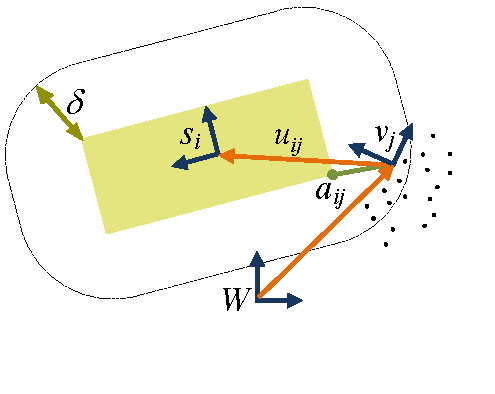
\includegraphics[width=5cm]{resources/model}}
\caption[Contact model]{Contact model. The figure shows the $i$-th link $\rl_i$ (solid block) and its pose $s_i$. The black dots are samples of the surface of an object. The distance $a_{ij}$ between a feature $v_j$ and the closest point on the link's surface is shown. The rounded rectangle illustrates the cut-off distance $\delta_i$. The poses $v_j$ and $s_i$ are expressed in the world frame $W$. The arrow $u_{ij}$ is the pose of $\rl_i$ relative to the frame for the surface feature $v_j$.}
\label{fig:representations.model}
\end{figure}

The parameters $\lambda$ and $\sigma_{p}$, $\sigma_{q}$, $\sigma_{r}$ were chosen empirically and kept fixed in all experiments reported in \sect\ref{sec:method}. The time complexity for learning each contact model from an example grasp is $\Omega(T K_O)$ where $T$ is the number of triangles in the tri-mesh describing the hand links, and $K_O$ is the number of points in the object model.


%\begin{figure}[t]
%\centering{
%\subfloat[]{\includegraphics[height=3.4cm]{resources/example1}}\quad
%\subfloat[]{\includegraphics[height=3.4cm]{resources/example2}}\quad
%\subfloat[]{\includegraphics[height=3.4cm]{resources/example5}}
%}
%\caption[Hand-object contact]{Example top grasp of a mug represented by a point cloud (panel a). The dotted regions are rays between features and the closest hand link surfaces (panel b). The black curves with frames at the fingertips represent the range of hand configurations in \eq\eqref{eq:hc} (panel c).}
%\label{fig:representations.modeldist.cont}
%\end{figure}

\subsection{Hand Configuration Model}

The hand configuration model, denoted by $\hc$, encodes a set of configurations of the hand joints $h_c \in \mathbb R^D$ (i.e., joint angles), that are particular to a grasp example. The purpose of this model is to allow us to restrict the grasp search space (during grasp transfer) to hand configurations that resemble those observed while training the grasp.

In order to boost the generalisation capability of the grasping algorithm the hand configuration model encodes the hand configuration that was observed when grasping the training object, but also a set of configurations recorded during the approach towards the object. Let us denote by $h^t_c$ the joint angles at some small distance \emph{before} the hand reached the training object, and by $h^g_c$ the hand joint angles at the time when the hand made contact with the training object. We consider a set of configurations interpolated between $h^t_c$ and $h^g_c$, and extrapolated beyond $h^g_c$, as
\begin{equation}
h_c(\gamma) = (1 - \gamma)h^g_c + \gamma h^t_c
\label{eq:learning.configmodel.config}
\end{equation}
\noindent where $\gamma \in \mathbb R$. For all $\gamma < 0$, configurations $h_c(\gamma)$ are beyond $h^g_c$ (see \fig\ref{fig:representations.modeldist.cont}). The hand configuration model $\hc$ is constructed by applying kernel density estimation to \begin{equation}\label{eq:H_c}\mathcal H_c = \lbrace h_c(\gamma): \gamma \in [-\beta, \beta], \beta \in \mathbb R^{+}\rbrace,\end{equation} as 
\begin{equation}
\hc(h_c) \equiv \sum_{\gamma \in [-\beta, \beta]} w({h_c(\gamma)}) \mathcal{N}_D(h_c|h_c(\gamma), \sigma_{h_c}) 
\label{eq:hc}
\end{equation}
where  $w({h_c(\gamma)}) = \exp(-\alpha \|h_c(\gamma) - h^g_c \|^2)$ and $\alpha \in \mathbb R^{+}$. $\alpha$ and $\beta$ were hand tuned and kept fixed in all the experiments. The hand configuration model computation has time complexity $\Omega(d_h K_C)$ where $d_h$ is the number of dimensions of the configuration vector, and $K_C$ is the size of the set of values of $\gamma$ used in \eq\eqref{eq:hc}.

\subsection{Reach to Grasp Trajectory}

We encode a reach to grasp trajectory as the combined trajectory of the wrist pose and the hand configuration. Each wrist pose is defined in the frame of reference of the final wrist pose in the trajectory. This final wrist pose is associated with the final hand configuration model and the contact models. We refer to the final hand configuration model, wrist pose and contact models as the model of the final grasp state.  A set of reach to grasp trajectories, including the final grasp states can be defined. We create this set so that the final grasp states are all very close to one another, thus forming an attractor, with the trajectories leading to those similar final grasp states defining an attractor basin.
